
\documentclass[a4paper, 10pt]{article}
\usepackage{a4wide}
\usepackage {amsmath}
\usepackage {graphicx}
\usepackage[utf8]{inputenc} 
\usepackage[francais]{babel}
\usepackage{fancyhdr}
\usepackage{setspace}
\usepackage{fancyhdr}
\usepackage{lastpage}
\usepackage{extramarks}
\usepackage{chngpage}
\usepackage[usenames,dvipsnames]{color}
\usepackage{graphicx,float,wrapfig}
\usepackage{ifthen}
\usepackage{listings}
\usepackage{courier}
\usepackage{braket}
\usepackage{MnSymbol,wasysym}
\usepackage{marvosym}
\usepackage{dsfont}
\usepackage{stmaryrd}
\usepackage{wrapfig}
\usepackage{enumitem}

\lhead{} 
\chead{} 
\rhead{\bfseries Intégration Numérique} 
\lfoot{JC Toussaint}
%\cfoot{} 
%\rfoot{\thepage}

% This is the color used for MATLAB comments below
\definecolor{MyDarkGreen}{rgb}{0.0,0.4,0.0}

% For faster processing, load Matlab syntax for listings
\lstloadlanguages{Matlab}%
\lstset{language=Matlab,                        % Use MATLAB
        frame=single,                           % Single frame around code
        basicstyle=\small\ttfamily,             % Use small true type font
        keywordstyle=[1]\color{Blue}\bf,        % MATLAB functions bold and blue
        keywordstyle=[2]\color{Purple},         % MATLAB function arguments purple
        keywordstyle=[3]\color{Blue}\underbar,  % User functions underlined and blue
        identifierstyle=,                       % Nothing special about identifiers
                                                % Comments small dark green courier
        commentstyle=\usefont{T1}{pcr}{m}{sl}\color{MyDarkGreen}\small,
        stringstyle=\color{Purple},             % Strings are purple
        showstringspaces=false,                 % Don't put marks in string spaces
        tabsize=5,                              % 5 spaces per tab
        breaklines=true,                        % Wrap long lines instead of overflowing
        breakatwhitespace=true,                 %
        %
        %%% Put standard MATLAB functions not included in the default
        %%% language here
        morekeywords={xlim,ylim,var,alpha,factorial,poissrnd,normpdf,normcdf},
        %
        %%% Put MATLAB function parameters here
        morekeywords=[2]{on, off, interp},
        %
        %%% Put user defined functions here
        morekeywords=[3]{FindESS, homework_example},
        %
        morecomment=[l][\color{Blue}]{...},     % Line continuation (...) like blue comment
        numbers=left,                           % Line numbers on left
        firstnumber=1,                          % Line numbers start with line 1
        numberstyle=\tiny\color{Blue},          % Line numbers are blue
        stepnumber=5                            % Line numbers go in steps of 5
        }

% Includes a MATLAB script.
% The first parameter is the label, which also is the name of the script
%   without the .m.
% The second parameter is the optional caption.
\newcommand{\matlabscript}[2]
  {\begin{itemize}\item[]\lstinputlisting[caption=#2,label=#1]{#1.m}\end{itemize}}

\pagestyle{fancy}

\begin{document}

\title{Intégration numérique sur un maillage éléments finis 2D \\
Application au calcul des caractéristiques géométriques d'une section plane}

\author{Jean-Christophe Toussaint\\
%  Phelma\\
%\texttt{jean-christophe.toussaint@phelma.grenoble-inp.fr}
}
\date{\today}
 
\maketitle

Le but du B.E. est de calculer les caractéristiques géométriques d'une section plane $D$ de
forme quelconque -- son aire $S$, la position $(X_g, Y_g)$ de son centre de gravité $G$ et son
moment d'inertie $I_O$ par rapport à un point $O$ donné -- à partir d'une description
de $D$ par un maillage éléments finis triangulaire. Ces grandeurs interviennent par exemple
dans le calcul de la torsion ou de la flexion des poutres, où l'on a besoin des caractéristiques
géométriques de la section droite.

\section{Intégration d'une grandeur sur un domaine 2D}

Le domaine $D$ est ici bidimensionnel. On dispose d'un maillage éléments finis à base de
triangles décrivant $D$ (Fig.~\ref{geo}) : dans l'exemple qui servira de fil conducteur à ce
B.E., $D$ est un disque de rayon $R \simeq 1$, décrit par un maillage de $248$ noeuds et $432$
éléments triangulaires (fichier \tt{disk248.pro}\rm).

\begin{figure}[ht]
\begin{center}$
\begin{array}{c}
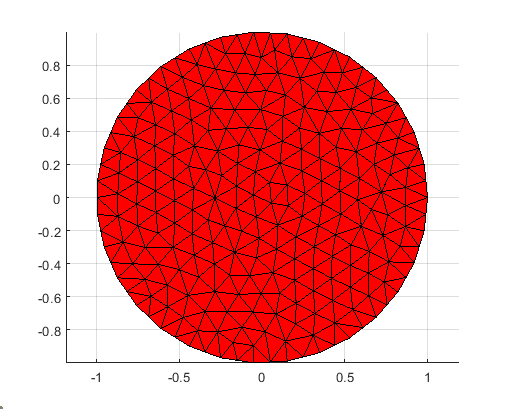
\includegraphics[scale=2, width=8cm]{disk_mesh.png}
\end{array}$
\end{center}
\label{geo} 
\caption{maillage triangulaire (T3) du disque décrit par \tt{disk248.pro}\rm : 248 noeuds, 432 éléments}
\end{figure}



La description d'un maillage en éléments finis se fait, de manière générale, par 
l'intermédiaire de deux tableaux, la table des coordonnées et la table de connectivité.


Dans ce B.E., on cherchera à calculer successivement l'intégrale de $4$ fonctions particulières,
qui donnent respectivement l'aire de $D$, les moments statiques permettant de localiser le
centre de gravité $G$ de $D$, et le moment quadratique polaire de $D$ par rapport à un point
$O(X_O, Y_O)$ quelconque:
\begin{equation}
S=\iint\limits_{D}\, dx\, dy \qquad\qquad
M_x=\iint\limits_{D}\, x\, dx\, dy \qquad\qquad
M_y=\iint\limits_{D}\, y\, dx\, dy
\end{equation}
\begin{equation}
I_O=\iint\limits_{D}\, \left[(x-X_O)^2+(y-Y_O)^2\right]\, dx\, dy
\end{equation}
Le centre de gravité $G(X_g, Y_g)$ de $D$ est alors donné par $X_g=M_x/S$ et $Y_g=M_y/S$, et le
théorème de Huygens (transport du moment quadratique polaire) relie le moment quadratique
$I_O$ calculé par rapport à un point $O$ quelconque au moment quadratique $I_G$ calculé par
rapport au centre de gravité $G$ :
\begin{equation}
I_O = I_G + S \cdot \overline{OG}^2
\label{huygens}
\end{equation}

Pour calculer l'intégrale élémentaire $I_e=\iint\limits_e f(x,y)\, dx\, dy$ sur un élément donné
$e$, on lui associe un élément de référence $e_{ref}$ (le triangle de sommets
$(0,0), (1,0), (0,1)$, de coordonnées locales $(u,v)$).
\begin{equation}
I_e=\iint\limits_e {f(x,y)\,dx\,dy} = \iint\limits_{e_{ref}} f(x(u,v), y(u,v))\, \det J(u,v)\, {du}\,  dv
\end{equation}
où
$
\det J(u,v)=
\left|
\begin{array}{rr} \partial_u x  & \partial_v x \\ \partial_u y  & \partial_v y \\ \end{array}
\right|  
$.\\

Il faut ensuite définir la transformation géométrique $T$ pour passer de l'élément de référence
à l'élément réel. La plus simple est une transformation isoparamétrique : les mêmes polynômes de
Lagrange $\alpha_{ie}(u,v)$, associés à chaque noeud $ie$ de l'élément, servent à interpoler les
coordonnées réelles à partir des coordonnées $(x_{ie}, y_{ie})$ des noeuds de l'élément:
\begin{equation}
\left\{ {\begin{array}{*{20}{c}}
 x(u,v)=\sum_{ie=I}^{NBN} x_{ie}\, \alpha_{ie}(u,v) \\ \\
y(u,v)=\sum_{ie=I}^{NBN} y_{ie}\, \alpha_{ie}(u,v)  
\end{array}} \right.
\label{isopara}
\end{equation}

Contrairement à un calcul d'éléments finis classique, où l'on interpole une grandeur physique
échantillonnée aux noeuds du maillage, la fonction $f(x,y)$ à intégrer ici ($f=1$, $f=x$, $f=y$
ou $f=(x-X_O)^2+(y-Y_O)^2$) est une fonction analytique connue des coordonnées réelles. Il
suffit donc, en chaque point d'intégration, de connaître les coordonnées réelles $(x,y)$ de ce
point --~obtenues directement par l'équation~\eqref{isopara}~-- pour pouvoir y évaluer $f$; on
n'a pas besoin, ici, d'interpoler une grandeur nodale.

L'estimation de l'intégrale élémentaire $I_e$ est alors calculée numériquement en utilisant la
méthode de Gauss:
\begin{equation}
I_e=\iint\limits_{e_{ref}} f(x(u,v),y(u,v))\, detJ(u,v)\,  du \,  dv= \sum_{k=1}^{NPI} f(x_k, y_k)\, w_k \, detJ(u_k, v_k)
\label{Ie_expr}
\end{equation}
où $(x_k, y_k)=(x(u_k,v_k), y(u_k,v_k))$ sont les coordonnées réelles, obtenues par
l'équation~\eqref{isopara}, du $k^{ieme}$ point de Gauss $(u_k, v_k)$, et $w_k$ son poids.

Finalement, l'intégrale sur tout le domaine $D$ est obtenue après assemblage de toutes
les intégrales élémentaires $I_e$ :
\begin{equation}
I = \sum_{e=1}^{NE} I_e
\end{equation}

\section{Implémentation}
\subsection {Structure de données}

La structure $ \tt{fem }\rm$ contient la description complète du maillage. $ \tt{fem.NP }\rm$  et   $ \tt{fem.NE }\rm$ retournent respectivement le nombre total de noeuds et le nombre d'éléments, et $ \tt{fem.NRG}\rm$ le nombre de régions du maillage (ici $\tt{fem.NRG=1}\rm$, le disque ne comportant qu'une seule région).

La table de coordonnées est implémentée sur la forme du tableau $ \tt{fem.noeud(1:fem.NP)} \rm$.
L'abscisse du noeud $\tt{np \in [1,   fem.NP \rm]}$ est donné par $ \tt{fem.noeud(np).x} \rm$ et son
ordonnée par $ \tt{fem.noeud(np).y} \rm$

Le tableau $\tt{fem.elt(1:fem.NE)} \rm$ contient pour chaque élément $ \tt{ne}\rm$ :

\begin{itemize}
\renewcommand\labelitemi{\textbullet}
\item sa dimension $\tt{fem.elt(ne).TYP} \rm$ (1 : élément linéique, 2 : élément surfacique -- dans \tt{disk248.pro}\rm, les 432 éléments sont tous surfaciques),
\item  son nombre de noeuds $\tt{fem.elt(ne).NBN} \rm$ (NBN=3 pour un triangle T3),
\item le numéro de région $\tt{fem.elt(ne).NRG} \rm$ auquel l'élément $ne$ appartient  et
\item  sa table de connectivité $\tt{fem.elt(ne).ind(ie)} \rm$ avec $\tt{ie \in [1,   fem.elt(ne).NBN \rm]}$
\end{itemize} 

Enfin, les coordonnées $(X_O, Y_O)$ du point $O$ par rapport auquel on souhaite calculer le
moment quadratique polaire sont stockées dans $\tt{fem.Xo}\rm$ et $\tt{fem.Yo}\rm$.

Les données nécessaires pour le programme, c'est à dire uniquement ici le maillage (le fichier
\tt{.pro}\rm{} contient également des sections \tt{AFFECTATION\_PROPRIETES\_PHYSIQUES}  et \\
\tt{CONDITIONS\_DIRICHLET}\rm{}, héritées d'un format de fichier commun à d'autres B.E., mais qui
ne sont pas utilisées ici), sont contenues dans le fichier d'extension $\tt{.pro} \rm$. La
lecture est effectuée par la fonction $\tt{lecture\_probleme.m} \rm$

%\matlabscript{lecture_probleme}{lecture des données du problème}

La fonction $\tt{femutil.m}\rm$, appelée juste après la lecture du maillage, parcourt l'ensemble
des noeuds pour en déduire la boîte englobante du domaine ($\tt{fem.xmin}\rm$,
$\tt{fem.xmax}\rm$, $\tt{fem.ymin}\rm$, $\tt{fem.ymax}\rm$) ainsi qu'une longueur caractéristique
$\tt{fem.lc}\rm$, utiles notamment pour l'affichage.

%\matlabscript{femutil}{caractérisation du maillage (boîte englobante)}

Deux fonctions permettent de visualiser le maillage lu. $\tt{affichage\_maillage.m}\rm$ trace le
maillage en numérotant chaque noeud et chaque élément (en distinguant, par un code couleur, les
éléments linéiques et surfaciques); elle n'est utilisable en pratique que sur des maillages de
petite taille (quelques dizaines d'éléments), utiles en phase de mise au point.

%\matlabscript{affichage_maillage}{affichage du maillage avec numérotation des noeuds et des éléments}

Pour un maillage de plus grande taille comme \tt{disk248.pro}\rm{} (432 éléments), on préfère
utiliser $\tt{affichage\_region.m}\rm$, qui colorie chaque région du maillage (ici l'unique
région du disque) à l'aide d'une couleur obtenue par la fonction $\tt{rgb.m}\rm$ (qui reproduit
une échelle de couleurs de type \tt{jet}\rm). C'est cette fonction qui est appelée par le
programme principal.

%\matlabscript{affichage_region}{affichage colorié des régions du maillage}

\subsection {polynomes de Lagrange sur le triangle à trois noeuds}

Pour chaque élément $\tt{ne} \rm$, la fonction $\tt{polynomes\_T3.m} \rm$ retourne une structure
de données $\tt{gauss} \rm$. Celle-ci contient, pour chacun des $\tt{gauss.NPI} \rm$ points
d'intégration de Gauss, le poids associé $\tt{gauss.pds(npi)}\rm$ et la valeur du déterminant
jacobien $\tt{gauss.detJ(npi)}\rm$. Elle retourne également, ce qui est essentiel pour ce B.E.,
les coordonnées réelles $\tt{gauss.x(npi)}\rm$ et $\tt{gauss.y(npi)}\rm$ de chaque point de
Gauss, calculées à partir de la transformation isoparamétrique~\eqref{isopara}.

%\matlabscript{polynomes_T3}{polynomes de Lagrange et coordonnées réelles des points de Gauss}

\section {Travail à réaliser}

La fonction $\tt{integrale.m}\rm$ ci-dessous, à compléter (les lignes manquantes sont repérées
par le commentaire \tt{\% A COMPLETER}\rm), doit calculer, sur l'élément $\tt{ne}\rm$, les quatre
grandeurs élémentaires $S_e$, $I_{x_e}$, $I_{y_e}$ et $I_{r^2_e}$ conformément à
l'équation~\eqref{Ie_expr}, en utilisant successivement $f(x,y)=1$, $f(x,y)=x$, $f(x,y)=y$ puis
$f(x,y)=(x-X_O)^2+(y-Y_O)^2$.

%\matlabscript{integrale}{intégrale élémentaire (à compléter)}

Ces contributions élémentaires sont ensuite assemblées, sur tous les éléments du maillage, par
la fonction $\tt{solution.m}\rm$ (fournie, elle ne demande pas de modification) pour obtenir
$S$, $X_g$, $Y_g$ et $I_O$:

%\matlabscript{solution}{assemblage des contributions élémentaires}

Les tâches à réaliser sont :

\begin{enumerate}
\item  Comprendre la structure du fichier $\tt{disk248.pro} \rm$ et le rôle des fonctions
$\tt{lecture\_probleme.m}\rm$, $\tt{femutil.m}\rm$, $\tt{affichage\_maillage.m}\rm$ et
$\tt{affichage\_region.m}\rm$ fournies.
\item Comprendre la fonction $\tt{polynomes\_T3.m}\rm$, et en particulier la façon dont les
coordonnées réelles $\tt{gauss.x(npi)}\rm$ et $\tt{gauss.y(npi)}\rm$ de chaque point de Gauss
sont obtenues à partir de la transformation isoparamétrique~\eqref{isopara}.
\item Compléter la fonction $\tt{integrale.m} \rm$ pour qu'elle calcule les quatre grandeurs
élémentaires $S_e$, $I_{x_e}$, $I_{y_e}$ et $I_{r^2_e}$ selon l'équation~\eqref{Ie_expr}.
\item Comprendre la fonction $\tt{solution.m}\rm$, qui somme les contributions de toutes les
intégrales élémentaires pour obtenir $S$, $X_g$, $Y_g$ et $I_O$.
\item Exécuter le programme principal $\tt{Moment\_main.m} \rm$ sur le maillage
$\tt{disk248.pro}\rm$ (disque de rayon $R\simeq 1$) et calculer successivement $I_O$ par rapport
à l'origine $O(0,0)$, par rapport au centre de gravité $G$, puis par rapport à un point
$D(0,-1)$. Comparer $S$ et $I_O$ (par rapport à l'origine) aux valeurs analytiques d'un disque
plein de rayon $R$ ($S=\pi R^2$, $I_O=\pi R^4/2$), et commenter l'écart observé, dû à
l'approximation du contour du disque par des segments de droite.
\item Vérifier numériquement, à partir des résultats obtenus à la question précédente pour $I_G$
et $I_D$, le théorème de Huygens~\eqref{huygens} reliant $I_D$ à $I_G$.
\item  La fonction $\tt{polynomes\_T3.m} \rm$ utilise $3$ points de Gauss. En examinant le degré,
en $(u,v)$, des quatre fonctions $f(x(u,v),y(u,v))\cdot detJ(u,v)$ associées à $S_e$, $I_{x_e}$,
$I_{y_e}$ et $I_{r^2_e}$ (on rappelle que, pour un triangle à 3 noeuds, $x(u,v)$, $y(u,v)$ et
$detJ(u,v)$ sont des fonctions affines et donc que $detJ$ est constant sur l'élément), discuter
si ce choix de $3$ points de Gauss est nécessaire pour obtenir un résultat exact sur chacune des
quatre grandeurs, ou si un nombre de points inférieur suffirait pour certaines d'entre elles.
\end{enumerate} 

%\matlabscript{Moment_main}{programme principal}

\end{document}

